% ============================================================================================
% This is a LaTeX template used for the course
%
%  I M A G E   B A S E D   B I O M E T R I C S
%
% Faculty of Computer and Information Science
% University of Ljubljana
% Slovenia, EU
%
% You can use this template for whatever reason you like.
% If you have any questions feel free to contact
% ziga.emersic@fri.uni-lj.si
% ============================================================================================

\documentclass[9pt]{IEEEtran}

% basic
\usepackage[english]{babel}
\usepackage{graphicx,epstopdf,fancyhdr,amsmath,amsthm,amssymb,url,array,textcomp,svg,listings,hyperref,xcolor,colortbl,float,gensymb,longtable,supertabular,multicol,placeins}

 % `sumniki' in names
\usepackage[utf8x]{inputenc}

 % search and copy for `sumniki'
\usepackage[T1]{fontenc}
\usepackage{lmodern}
\input{glyphtounicode}
\pdfgentounicode=1

% tidy figures
\graphicspath{{./figures/}}
\DeclareGraphicsExtensions{.pdf,.png,.jpg,.eps}

% correct bad hyphenation here
\hyphenation{op-tical net-works semi-conduc-tor trig-gs}

% ============================================================================================

\title{\vspace{0ex} %
Ear Detector
\\ \large{Assignment \#2}\\ \normalsize{Image Based Biometrics 2020/21, Faculty of Computer and Information Science, University of Ljubljana}}
\author{ %
Jan~Joneš
\vspace{-4.0ex}
}

% ============================================================================================

\begin{document}

\maketitle

\begin{abstract}
In this report, I describe results of developing an ear detector.
First I describe detector architecture.
Then I present performance results.
\end{abstract}

\section{Introduction}
I developed a convolutional neural network (CNN) that can segment ears pixel-wise.
This network is intended for use in biometric pipeline.
The architecture has been developed from scratch based on my knowledge from deep learning course~\cite{npfl114}.
For training and evaluation, I have used AWE dataset~\cite{awe}.
Source code of both the model and this report can be found in GitHub repository~\cite{repo}.

\section{Methodology}
Praesent at mollis diam. Suspendisse fringilla feugiat porttitor~\cite{neuro2008,neuro2013}. Donec accumsan non libero sed rutrum. In maximus cursus mauris, eget consectetur purus semper vel. Vivamus non dictum nisi. Duis et quam nec lacus faucibus porttitor. Suspendisse potenti. In dignissim blandit viverra. Proin aliquam vulputate nisl ac sollicitudin.

 Suspendisse et quam eget dui commodo aliquet. Nunc eu sagittis tellus, non faucibus velit. Quisque in tempus turpis, non placerat elit. Sed vitae imperdiet felis~\cite{Jain2004,Jain2011}.

Proin at dolor at enim aliquet dignissim eget id ante. Cras quis magna a lorem posuere lacinia eget quis felis. Vestibulum consequat lacinia justo a elementum. Morbi sed placerat dolor. Duis urna massa, venenatis quis tincidunt feugiat, interdum eu tellus. Mauris ullamcorper, arcu sit amet fringilla scelerisque, lacus lectus vehicula ipsum, eu lacinia mauris dolor a arcu.

In ut arcu eget nisl maximus blandit a vitae elit. Nulla laoreet est eu sapien blandit luctus. Suspendisse quis porttitor leo. Class aptent taciti sociosqu ad litora torquent per conubia nostra, per inceptos himenaeos. Suspendisse volutpat sem risus, facilisis laoreet leo rhoncus ac. Etiam non quam felis. Vestibulum vel magna imperdiet, faucibus turpis vel, sagittis dolor.

\section{Results}
Nulla sodales, metus at faucibus iaculis, felis risus pulvinar erat, in pretium arcu ex sed elit. Cras ultrices felis in diam dictum interdum. Praesent in interdum dolor, ut varius massa. Integer non efficitur risus, nec dapibus dui. Nunc sollicitudin nibh in orci pretium, quis congue ligula faucibus. Vivamus fermentum leo ac euismod porta as shown in Figure~\ref{fig:plot1}.

\begin{figure}[h]
    \centering
    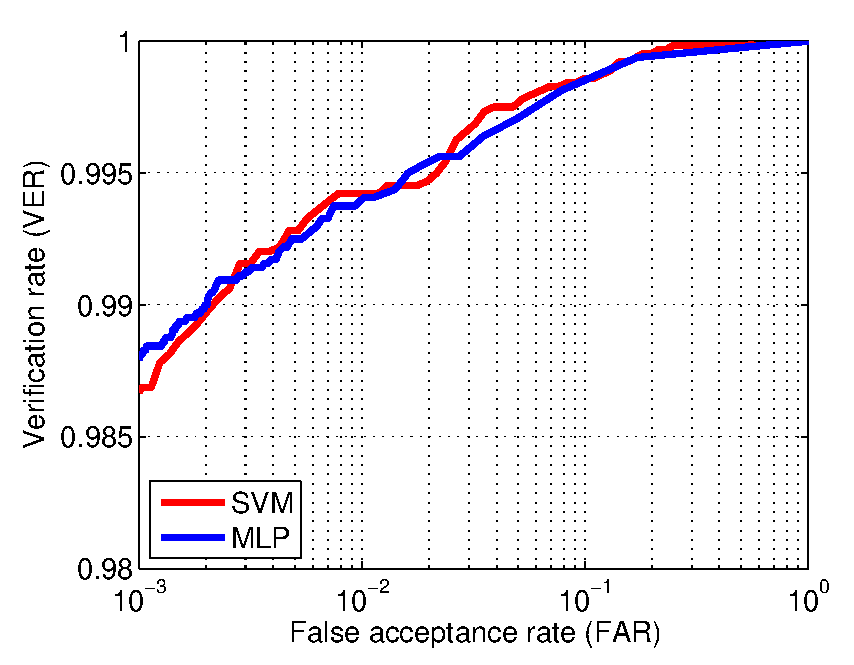
\includegraphics[width=1\columnwidth]{plot1}
    \caption{A nice plot showing something really cool and awesome.}
    \label{fig:plot1}
\end{figure}
 
Sed et enim non justo mattis finibus sed at felis. Phasellus vel nibh vehicula, consectetur lectus in, bibendum enim. Nam rutrum suscipit magna id maximus. Quisque posuere lorem vel ante viverra, ut euismod sapien pulvinar. Fusce vitae maximus nibh. Sed dignissim dignissim nunc eu finibus. In pulvinar purus nisl, et mattis magna pretium ac. Curabitur nec massa vel est eleifend cursus nec sed elit. Vestibulum at nibh felis. Sed porttitor ut turpis in tristique.

 \section{Conclusion}

Aenean tincidunt sodales ante et egestas. Nam consectetur nunc iaculis tincidunt egestas. Vivamus sagittis mi et vehicula facilisis. Phasellus semper volutpat gravida. Vestibulum vitae neque sed purus pharetra suscipit eget mollis dui. Morbi lobortis justo a lacus feugiat, et finibus eros tristique.

\bibliographystyle{IEEEtran}
\bibliography{bibliography}

\end{document}
